\documentclass[DM,lsstdraft,toc]{lsstdoc}

\usepackage[english]{babel}
\usepackage[utf8x]{inputenc}
\usepackage{amsmath}
\usepackage{graphicx}
\usepackage{longtable}
\usepackage{hyperref}
\usepackage{comment}
\usepackage{natbib}

\excludecomment{changelog}
\excludecomment{todo}
\excludecomment{openissues}

% Local commands go here
\newcommand{\G}[1]{{\color{green} #1}}
\newcommand{\B}[1]{{\color{blue} #1}}
\newcommand{\R}[1]{{\color{red} #1}}

%% Journal abbreviations
\bibliographystyle{aasjournal}

\title[LSST Science Platform]{LSST Science Platform Vision Document}

\author{
M.~Juri\'c,
D.~Ciardi,
and
G.P.~Dubois-Felsmann
}

\setDocRef{LDM-nnn}
\date{\today}
\setDocRevision{1.0}
\setDocStatus{draft}

\setDocAbstract{%

This document defines the high-level vision for the {\bf LSST Science
Platform (LSP)}, a set of web applications and services through which the
the scientific community will to access, visualize, interact with,
and analyze LSST data holdings.
\\

It is meant to inform the development of requirements, product specifications,
prioritization, and plans for the elements of the DM system that together comprise
the LSP.

}

% Change history defined here. Will be inserted into
% correct place with \maketitle
% OLDEST FIRST: VERSION, DATE, DESCRIPTION, OWNER NAME
\setDocChangeRecord{%
\addtohist{1}{2017-03-15}{Initial high-level description of the concept}{Mario Juric}
%\addtohist{2}{yyyy-mm-dd}{Future changes}{Future person}
}

\begin{document}

% Create the title page
% Table of contents will be added automatically if "toc" class option
% is used.
\maketitle

\section{Introduction}

\subsection{Goals and Philosophy}

The LSST is a facility whose primary mission is to acquire, process, and
make available the data collected by its telescope and camera, as well as
enable ``next-to-the-data'' creation of added-value (Level 3) data products
\cite{SRD}.

This document describes the vision for the services to be put into place to
fulfill the ``{\em making available}'' and ``{\em Level 3} creation``
aspects of LSST's mission; its aim is to present a high-level
description of the data access and analysis services provided at the
LSST Data Access Centers.

\subsection{LSST Science Platform Overview}

\begin{figure}
\centering
\scalebox{0.4}{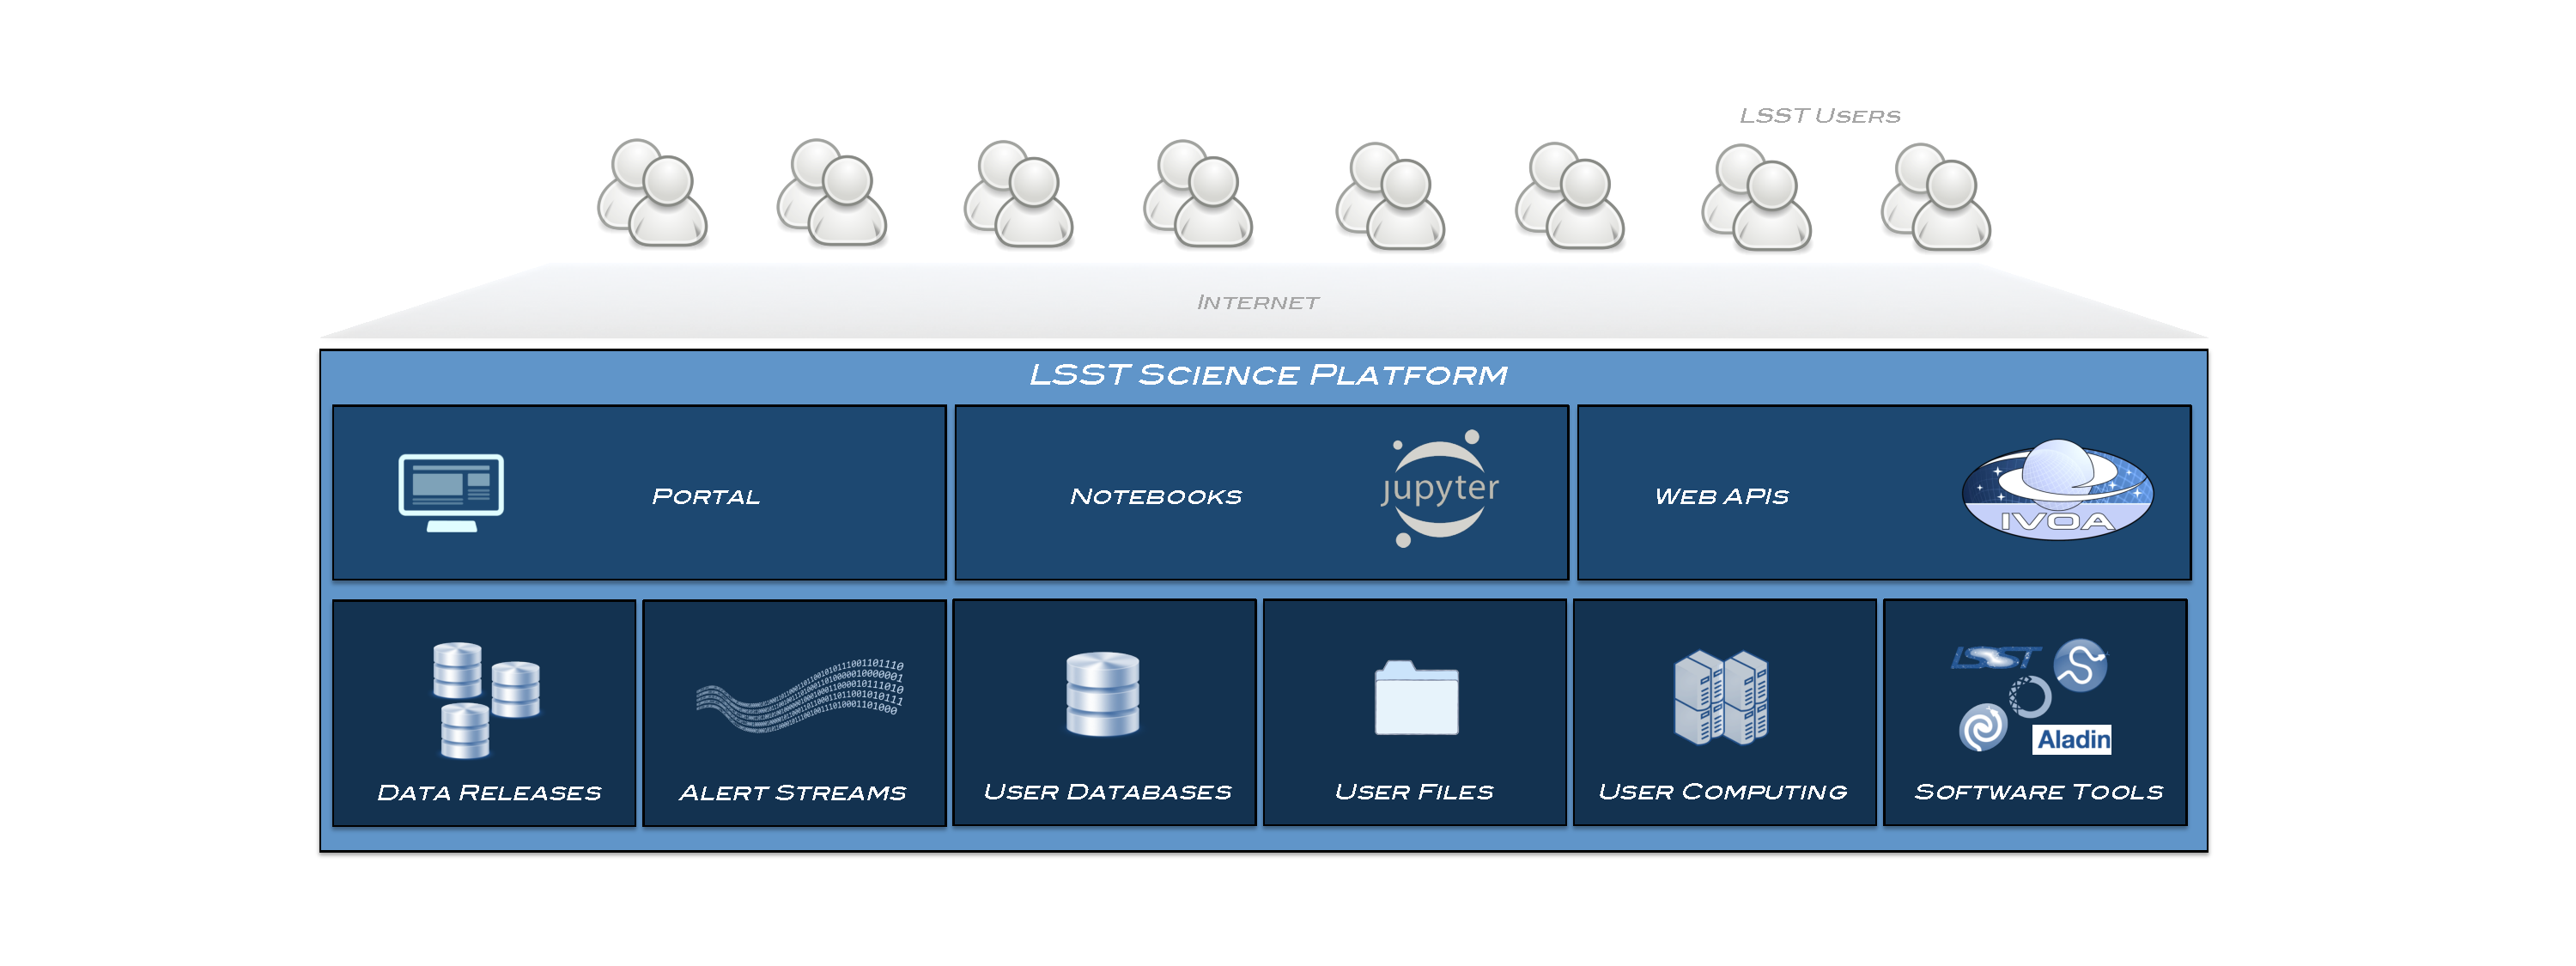
\includegraphics[trim={5cm 0.5cm 3cm 0.5cm},clip,page=1]{images/fig-lsst-science-platform-extended.pdf}}
\caption{
A high-level, layered, view of the LSST Science Platform.  The LSST data
will be exposed to the users through the web Portal, the Jupyter Notebook
interface, and machine-accessible Web APIs.  The web Portal component will
provide the essential data access and visualization services common to
present day archives.  The Notebook component, based on the Jupyter family
of technologies (JupyterHub and JupyterLab) will allow for more
sophisticated next-to-the-data analysis.  These user-visible services will
provide acces to the underlying core LSST data sets -- the data releases and
alert streams -- and be supported by the user Database, File Storage,
Computing, and Software Tools components.  Together, they will enable the
users to access, sub-select, analyze, and perform added-value processing of
all flavors of LSST Data Products (see text for detail). 
\label{fig:layeredLSP}}
\end{figure}

We define the LSST Science Platform (LSP) as a set of web applications and
services made available to the scientific community to access, visualize,
subset, and perform next-to-the-data analysis of the LSST data set.  The
platform can be thought of as exposing three primary user-facing ``aspects''
-- the web Portal, the Notebook analysis environment, and a
machine-accessible Web API interface -- and a number of infrastructure
elements supporting its function.  (Figure~\ref{fig:layeredLSP}).

We imagine most (nearly all) LSST users will access LSST data products and
resources via the the Internet....

The Portal component is a web portal designed to provide the essential data
access and visualization services through a simple-to-use website.  It will
enable browsing and visualization of the available datasets in ways the
users are accustomed to at archives such as IRSA, MAST, or the SDSS archive,
with an enhanced level of interactivity in line with expectations for
then-contemporary archive portals.  Through the Portal, the users will be
able to view the LSST images, request subsets of data (via simple forms or
SQL queries), store the results of such queries to their personal
workspaces, construct commonly requested plots, and generally explore the
LSST dataset in a way that allows them to identify and access (subsets of)
data required by their science case.

The Notebook environment, based on the Jupyter family of technologies (e.g.,
JupyterHub and JupyterLab), will be provided to allow for more sophisticated
data selection, analysis, and creation of added value (Level 3) data
products.  The Notebook environment will come preinstalled with a library of
commonly used and useful software Tools (such as AstroPy, LSST software
stack, Anaconda Scientific Python Distribution, and others).  The users will
be able to upload and install their own tools as well.

The Notebook user experience will be nearly identical to working with
Jupyter notebooks locally, except that computation and analysis will occur
at resources provided at the LSST Data Access Center.  This is an
implementation of the “bringing computation to the data” paradigm: rather
than imposing the burden of downloading, storing, and processing (large)
subsets of LSST data at their home institutions, we will enable our users to
bring their codes and perform their analysis at the LSST DAC.  We expect
this will reduce the barrier to entry and shorten the path to science for
the LSST science community.

Queries, visualizations, and analysis performed through the Portal and
Notebooks will be served by a shared computing cluster, file storage, and
database resource (bottom row of Figure~\ref{fig:layeredLSP}).  At start of operations,
this computing cluster will number 2,400 cores (approximately 18 TFLOPs),
with 4 PB of file and 3 PB of database storage (numbers for the U.S.  DAC). 
These will be shared by all users, the number of whom we’re estimating in
the low thousands.

Not all users will be accessing the computing cluster concurrently; though
difficult to predict with accuracy because of a lack of direct comparables,
an estimate on order of a ~100 concurrent users is likely reasonable.  This
would translate to typical allocations of ~20 cores per user, sufficient to
enable preliminary end-user science analyses (working on catalogs, smaller
number of images) and creation of some added-value (Level 3) data products. 
A good analogy is one of being given a server with a few TB of disk, few TB
of database storage, that is co-located next to the LSST data, and with a
chance to use tens to hundreds of cores for analysis (depending on system
load).

For larger endeavors (e.g., pixel-level reprocessing of the entire LSST
kdataset), the users will be steered towards resources beyond the LSST DACs
(e.g., national supercomputing centers, university computing centers, or the
public cloud).  Backend Science Platform services (including access to
databases, images, and other files) will be exposed through
machine-accessible web APIs serving community-accepted formats and
protocols.  This will make it easy to initiate remote computations operating
on LSST data.  Virtual Observatory interfaces will allow connection to other
archives and enable the use of standard tools such as TOPCAT or Aladin. 
This will further lower the barrier to access to LSST data, shortening the
path to science.

Finally, the LSST Science Platform is being designed to allow for
collaborative work.  The capabilities ranging from sharing of derived
datasets within smaller groups, collaborations, or with the broader LSST
community, to collaborative visualization and editing capabilities expected
to become available within the Jupyter ecosystem.

\section{Enabling Remote Data Access and Analysis}

\subsection{Web Portal}

\subsection{Jupyter Notebooks}

\subsection{Web APIs}

\section{Hosting Level 1 and 2: Database and Alert Filtering Services}

\subsection{Relational Databases}

\subsection{Alert Filtering Services}

\section{Enabling Level 3: User Databases, File storage, and Computing}

\subsection{Computing}

\subsection{File Storage}

\subsection{User Databases}

\end{document}
